\section{GAN在损失函数的改进}
GAN在2014年能被提出时, 是一个巧合, 当晚刚好训练出来了. 一般情况下, GAN难以训练. 其原因是GAN通过有限的采样来估计分布相似度JS Divergence作为损失函数估计, 而在有限的采样中, 数据重叠很少. 根据 JS Divergence公式为: 

\begin{equation}
    JSD(P||Q)=\frac{1}{2}\sum p(x)log(\frac{p(x)}{p(x)+q(x)}) + \frac{1}{2}\sum q(x)log(\frac{q(x)}{p(x)+q(x)}) + log2
\end{equation}

\subsection{f-GAN}
在数据重叠区域较少时, $JSD=log2$, 为定值, 没有梯度下降, 难以训练. 因此f-gan~\cite{f-gan}提出观点, 任何divergence都可以用来训练GAN. 其原文为:

\begin{quotation}
    \bfseries
    We show that the generative-adversarial approach is a special case of an existing more general variational divergence estimation approach. We show that any f-divergence can be used for training generative neural samplers. We discuss the benefits of various choices of divergence functions on training complexity and the quality of the obtained generative models.
\end{quotation}

其核心公式为: 
\begin{equation}
    D_{f}(P||Q)=\int_{x} q(x)f(\frac{p(x)}{q(x)}) dx
\end{equation}
要求$f(x)$为convex, 则可推出 $f(1)=0$. 即当$P$和$Q$分布相同时, $D_{f}(P||Q)$值最小为$0$. 当$f(x)=xlogx$时, 在数学上估计的是分布之间的KL divergence; 当$f(x)=-logx$时, 在数学上估计的是分布之间的Reverse KL divergence; 当$f(x)=(x-1)^{2}$时, 在数学上估计的是Chi Square. 

通过Fenchel Conjugate将不同的Divergence与GAN相联系. 每一个convex的$f(x)$都存在一个$f^{\star}$使:
\begin{equation}
    f^{\star}(t) = \max \limits_{x\in dom(f)} {xt-f(x)}
    \label{equ:0203}
\end{equation}
穷举所有$t$, 对每个$t$找到使$xt-f(x)$最大的$x_{max}$值, 使$f^{\star}(t) = x_{max}t-f(x_{max})$. 

\begin{align}
    D_{f}(P||Q) & = \int_{x}q(x)f(\frac{p(x)}{q(x)}) dx \\
    & = \int_{x}q(x)(\max \limits_{t\in dom(f^{\star})} (\frac{p(x)}{q(x)}t-f^{\star}(t)) dx  \\
    & \approx \max \limits_{D} \int_{x} p(x)D(x) dx - \int_{x} q(x)f^{\star}(D(x)) dx \label{eq:0206} \\
    & = \max \limits_{D}(E_{x\sim P}(D(x))-E_{x\sim Q}(f^{\star}(D(x))))
\end{align}
在上式中, $t$是标量, 在GAN里则为$D(x)$, 根据~\ref{equ:0203}, 可得上式~\ref{eq:0206}. 具体每一种Divergence对GAN的影响可见原论文. 

\subsection{LSGAN}
另外由于原始GAN的Discriminator最后一层是sigmoid, 训练时容易梯度消失, 因此LSGAN~\cite{LSGAN}改变了其损失函数, 如下式~\ref{eq:0208}与~\ref{eq:0209}所示, 其中$a, b, c$都是需要调整的超参数. $a, b$分别为假数据和真数据的标量, $c$是G想让D觉得是真数据的标量
\begin{equation}
    \min \limits_{D}V_{LSGAN}(D)=\frac{1}{2}E_{x\sim P_{data}}[D(x)-b]^{2} + \frac{1}{2}E_{x\sim P_{G}}[D(G(z))-a]^{2}
    \label{eq:0208}
\end{equation}

\begin{equation}
    \min \limits_{G}V_{LSGAN}(G)= \frac{1}{2}E_{x\sim P_{G}}[D(G(z))-c]^{2}
    \label{eq:0209}
\end{equation}

\subsection{WGAN}
在WGAN~\cite{WGAN}中, 使用动土距离(Earth Mover's Distance)来估计两种分布之间的差异, 比较详细的解释\href{https://vincentherrmann.github.io/blog/wasserstein/}{国外博客}, 如图~\ref{fig:0201}所示, 寻求两个分布之间转换的距离.
\begin{figure}[!htbp]
    \centering
    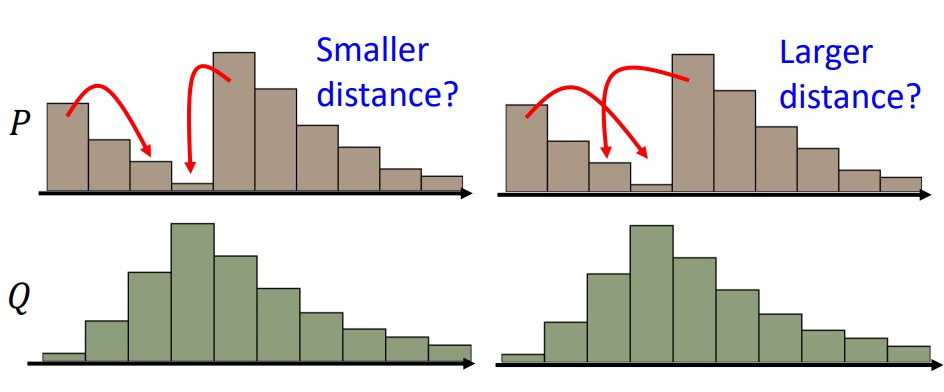
\includegraphics[height=12em]{pic/pic0201.jpg}
    \caption{动土距离示意图}
    \label{fig:0201}
\end{figure}

但这种转换的求解是不唯一的, 我们需要找的是总的转换距离最小的那个值作为最终的动土距离, 如图~\ref{fig:0202}所示:
\begin{figure}[!htbp]
    \centering
    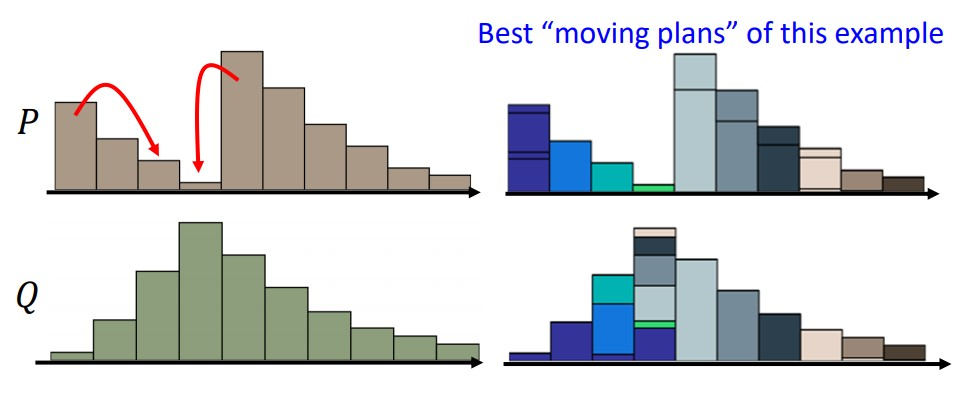
\includegraphics[height=12em]{pic/pic0202.jpg}
    \caption{动土距离求解}
    \label{fig:0202}
\end{figure}

对于转换方式$\gamma$的距离, 可通过矩阵表示每个转换方式$\gamma$, 如下式所示:
\begin{equation}
    B(\gamma) = \sum_{x_{p}, x_{q}} \gamma(x_{p}, x_{q})\Vert x_{p} - x_{q} \Vert
\end{equation}
则最终的动土距离$W(P,Q)$为
\begin{equation}
    W(P,Q) = \min \limits_{\gamma} B(\gamma)
\end{equation}

在图~\ref{fig:0203}中, 矩阵中的值代表其转移大小, 行标表示转移起点, 列标表示转移终点. 
\begin{figure}[!htbp]
    \centering
    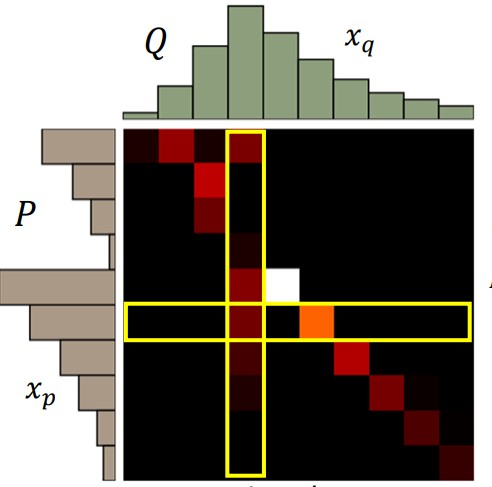
\includegraphics[height=12em]{pic/pic0203.jpg}
    \caption{动土距离公式图解}
    \label{fig:0203}
\end{figure}

相比原始GAN, 当使用动土距离去描述两个分布间差异时, 考虑了两个分布没有重叠的情况, 因此可以极大改善训练稳定性. WGAN将discriminator的损失函数设计为:

\begin{equation}
    V(G,D)=\max \limits_{D\in 1-Lipshcitz}(E_{x\sim P_{data}}[D(x)] - E_{x\sim P_{G}}[D(x)])
\end{equation}

并使用了weight-clipping.

% 其中$Lipshitz function$为:
% \begin{equation}
%     \Vert f(x_{1}) - f(x_{2}) \Vert \leq K \Vert x_{1} - x_{2} \Vert
% \end{equation}
% 当$K=1$时, 为$1-Lipshcitz$. 这样可以限制$V(G,D)$, 在不会造成梯度消失的情况下, 避免其值改变过快, 提升训练稳定性. 同时在梯度下降时, 使用weight clipping, 更保证训练稳定性.

\subsection{WGAN-GP}
WGAN-GP的作者认为, 由于weight clipping的存在, 会导致训练出现不正常现象, 在WGAN损失函数基础上, 加入了gradient penalty这个惩罚项. 

\begin{equation}
    V(G,D)=\max \limits_{D\in 1-Lipshcitz}(E_{x\sim P_{data}}[D(x)] - E_{x\sim P_{G}}[D(x)]) + \lambda E_{x\sim P_{penalty}}[(\Vert \nabla D_{x} \Vert - 1)^{2}]
\end{equation}

% \begin{figure}[!htbp]
%     \centering
%     \subfloat[BC]{\label{fig:0105a}
%     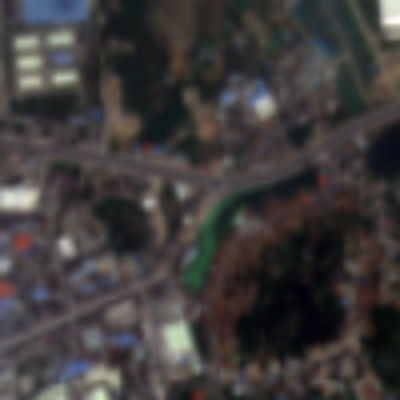
\includegraphics[height=10em]{pic/img5_LR_bicubic.jpg}}
%     \quad
%     \subfloat[SR]{\label{fig:0105b}
%     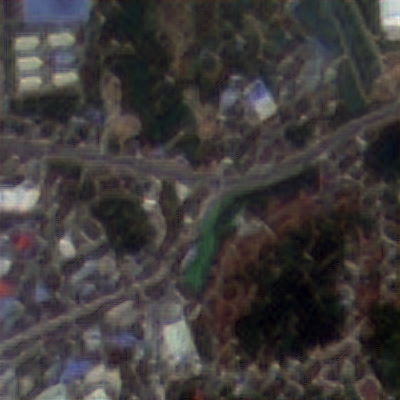
\includegraphics[height=10em]{pic/img5_SR.jpg}}
%     \quad
%     \subfloat[GT]{\label{fig:0105c}
%     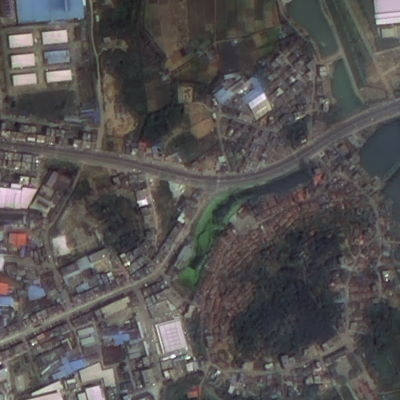
\includegraphics[height=10em]{pic/img5_GT.jpg}}
%     \caption{result05}
%     \label{fig:0105}
% \end{figure}